\documentclass[12pt]{article}
\usepackage{helvet}
\renewcommand{\familydefault}{\sfdefault}
\usepackage[letterpaper, top=1.2in, bottom=1.2in, left=1.2in, right=1.2in, heightrounded]{geometry}
\linespread {1.15}
\usepackage{graphicx}
\graphicspath{ {./assets/img} }
\author {Alexis Aoun}
\begin{document}
\begin {sloppypar}
\title {Stage Atos}
\date {}
\maketitle
\newpage

% 2 - missions
% MPP
\section {Objectifs et réalisation de mes missions}
\subsection {MPP Dashboard}
\subsubsection {Le contexte}
\paragraph {}
Atos a une plateforme en ligne, My Atos, sur laquelle tous les employés doivent 
renseigner leurs informations personnelles ainsi que leurs parcours professionel et 
académique. Le problème de cette procédure, qui est en théorie obligatoire, est qu' 
une partie importante des salariés ne remplissent pas ces informations, et la plupart 
du temps cela est dû à un simple oubli. Pour y remédier, le service RH et la direction 
général d'Atos décidèrent de lancer un projet interne qui permetterait de relancer 
les employés automatiquement à partir d'un fichier excel contenant les informations 
de tous les collaborateurs, fournit par le service RH. Ce projet fut baptisé MPP Dashboard.

\paragraph {} 
Le projet est une application web(TODO) dont le fonctionnement repose sur trois processus
principaux : 
\begin {enumerate}
  \item 
    Le traitement de l'excel : Le service RH fournit un fichier excel sous format XSLX 
    (Le format par défaut des fichiers excels microsoft). Celui-ci doit être traité de 
    manière à ce que les informations qu'il contient puissent être manipuler 
    programmatiquement.
  \item 
    Le filtrage : Une fois les donnés des collaborateurs dans notre application, on
    sauvegarde dans une base de donnée uniquement ceux dont le taux de renseignement 
    d'informations et en-dessous d'un seuil défini par les administrateurs de 
    l'application. Le taux par défaut est de 90\%. 
  \item 
    L'envoie de mail : L'application enverra des mails à tous les salariés présent 
    dans la base de données après la phase de filtrage. Un chiffre correspondant au nombre
    de mails envoyés au collaborateurs est associé à chacun d'entre eux. Au bout du 
    5ème mail l'employé n'ayant pas renseigner les informations nécéssaires est signalé 
    automatiquement au service RH.
\end{enumerate}
\newpage
\begin{figure}
  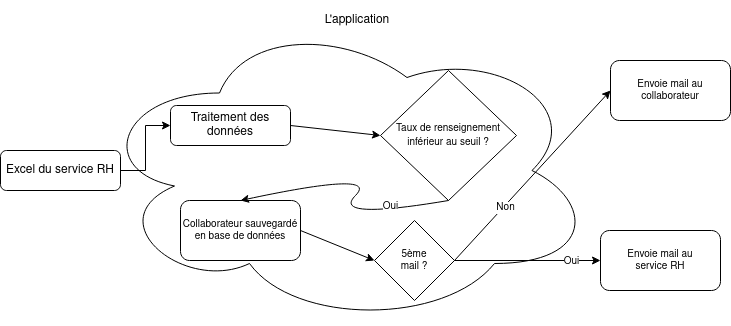
\includegraphics[width=\textwidth] {mpp-diagram.png}
  \caption {Diagram du fonctionnement de MPP Dashboard}
\end{figure}
\paragraph {}
Les technologies utilisés pour la réalisation du projet sont : 
\begin {itemize}
\item   
  Pour la base de données : PostgreSQL (TODO)
\item 
  Pour le serveur backend (TODO) : ExpressJS (TODO)
\item 
  Pour l'interface grahique : ReactJS (TODO)
\end {itemize}

\subsubsection{La problèmatique}
\paragraph {}
Lorsque je suis arrivé sur le projet, celui-ci a déjà été développé mais avait un 
problème avec l'un des processus, celui d'extraction de l'excel. En effet la librairie (TODO)
utilisée pour remplir cette tâche, du nom d'Excellente, a été développée en interne par des 
employés d'Atos et comporte certains inconvenients : 
\begin{itemize}
  \item 
    Il comporte plusieurs bugs (TODO). Cela est notamment dû au fait que cette librairie 
    n'est pas connue du grand publique et ne reçoit donc pas un grand nombre de tests et 
    de contributions 
  \item 
    La librairie devient exponentiellement lente avec la grandeur du fichier excel. Hors
    celui qu'on a à extraire fait plus de 40 000 lignes
\end{itemize}
Ma tâche est donc de trouver une solution qui puisse répondre à la fois aux problèmes
de vitesse et de fiabilité.
\newpage
\subsubsection{Les solutions possibles}
\paragraph {}
Afin d'accomplir ma mission j'ai étudié plusieurs possibilités : 
\begin{itemize}
  \item 
    Garder la librairie Excellente et essayer de gommer ces défauts en modifiant
    son implémentation, voir même la librairie en elle-même. 
    Le risque est que cela prenne trop de temps ou même que cela n'aboutisse tous 
    simplement pas. Du fait de l'utilisation limitée d'Excellente et du manque de documentation 
    techique, corriger la librairie pourrait prendre des mois alors que la direction d'Atos 
    attendait des résultats dans les semaines suivant mon arrivé.
  \item 
    Utiliser un script Python (TODO). Lors de mes différents cours en Data au sein de l'IMT Nord 
    Europe, l'une des compétences que j'ai acquis est le traitement de données par le biais 
    de script Python en utilisant des librairies tels que Panda (TODO). Les performances 
    seraient des ordres de grandeurs meilleurs que celle de n'importe quelle autre solution 
    implémentée en Javascript (TODO), et l'écriture du script peut se faire en une journée. 
    La difficulté est l'implémentation du pont entre le serveur ExpressJS et le script Python. 
    Celui-ci doit être exécuter au bon moment par le serveur, et ce dernier doit pouvoir 
    récupérer le résultat final. Il y avait aussi la problématique des dépendances(TODO) spécifique
    à Python dont a besoin un tel script qui rajouterait une couche de compléxité au projet ExpressJS, au 
    développement mais surtout à la maintenance.
  \item 
    Utiliser une autre librairie Javascript, ExcelJS(TODO). ExcelJS est sans aucun doute 
    la librairie Javascript la plus utilisée pour le traitement d'excel. Un avantage très important 
    d'une librairie aussi connue est sa documentation riche qui m'a permis de faire des premiers 
    tests rapidements. De ces expérimentations j'en avais conclu que la fiabilité était 
    satisfasante et que la vitesse était tout à fait convenable pour notre application, même si 
    plus lente que le script Python. Cette solution fut donc retenu.
\end{itemize}
\newpage
\subsubsection{La réalisation de la mission}
\paragraph{}
La mise en œuvre de la solution fut assez simple dans son ensemble en grande partie 
grâce à l'excellente documentation d'ExcelJS. La seule difficulté rencontrée a été la gestion 
des erreurs dans l'excel. En effet celui-ci comporte des formules qui dans certains cas retournent
des erreurs. Mon implémentation a donc dû prendre en compte ces cas de figures là. Après cela j'ai pu 
procéder à une série de tests sur mon ordinateur personnel, le traitement de l'excel comportant 40 000
lignes a duré dans les alentours des 1 minutes et 45 secondes. Il était temps de déployer ma solution 
en production.
\subsubsection{Résultats et bilan}
\paragraph{}
Après quelques ajustements mon algorithme de traitement obtenait les résultats escomptés.
Le temps d'exécution de moins de 2 minutes jugés satisfasant. 
\linebreak 
Avec plus de temps une implémentation du script Python aurait été possible, permettant de réduire encore
plus le temps de traitement. Néanmoins je pense avoir pu obtenir le meilleur résultat possible 
compte tenu de la contrainte temporelle.
\paragraph{}
Cette première mission fut l'opportunité pour moi de prouver à la fois mes compétences techniques
mais surtout mes capacités à prendre des initiatives et à les mettre en œuvre.
\end{sloppypar}
\end{document}

